\section{Relación con los clientes}
\subsection{Autoevaluación}
En esta sección se han cumplido los objetivos correspondientes al 10.
\subsection{Introducción}
\paragraph{}
En este apartado se va a realizar una gestión de las relaciones con los clientes en Odoo. Este factor es determinante para el éxito y la competitividad de la compañía. Se ofrecen varias herramientas y módulos dirigidos a la relación con los clientes que proporcionan la capacidad de captar, gestionar y cerrar acuerdos con clientes de manera eficiente. Se tiene como objetivo evaluar la idoneidad de Odoo como plataforma para este tipo de gestión.
\subsection{Metodología}
\paragraph{}
Para llevar a cabo la evaluación de esta sección se ha instalado los módulos CRM, Ventas y Facturación. A continuación, se han configurado estos módulos. Se ha activado la opción \textit{Leads} en los ajustes del módulo \textit{CRM}. Se ha establecido como divisa principal el Euro en los ajustes del módulo de Facturación.
\paragraph{}
El primer paso ha sido crear un equipo de ventas, para ello, se ha ido al módulo de ventas y se ha seleccionado la opción de \textit{Equipos de ventas}. Se ha creado un equipo de ventas llamado España que está formado por el usuario Pedro y James y tiene como líder del equipo a John. 
\paragraph{}
Por otro lado, se han creado 3 empresas cliente. Desde el módulo de ventas se ha hecho clic en el desplegable de pedidos y se ha seleccionado Clientes. Se ha creado la empresa cliente de origen español Zara, la cual durante el proceso de creación se han añadido 2 contactos en el apartado de Contactos y direcciones, Maria y Miguel. También, se ha creado el cliente Mercadona de origen español y se han añadido Pedro y Lucia como contactos de la empresa. Por otro lado, de origen suizo se ha creado como cliente la empresa de Nestle con los contactos de Theo y Francois. 
\paragraph{}
Durante el proceso de creación de cada empresa cliente se ha completado el campo de Condiciones de pago que se ubica en el panel de Venta y compra, en las empresas españolas se paga a 30 días  y las empresas suizas se paga a 45 días. En el mismo panel se ha asignado la Tarifa de las empresas españolas en Euros, mientras que en la empresa suiza se ha creado una nueva tarifa para que la lista de precios esté en Francos Suizos.
\paragraph{}
Desde la compañía nos hemos puesto en contacto con los clientes ofreciendo nuestro producto y como resultado, Mercadona y Zara se han mostrado interesados por lo que se han creado 2 iniciativas, una cada una de las empresas cliente. Para ello, desde el módulo \textit{CRM} en el menú de \textit{Leads} se han creado 2 entradas. Cada una se ha asignado a uno de los contactos de la empresa correspondiente y se ha establecido el ingreso esperado y la probabilidad que existe de que se convierta en oportunidad.
Además, desde la vista de Kanban del módulo de CRM se puede observar que se han añadido dos entradas en el apartado de nuevo.
\paragraph{}
La empresa de Mercadona nos ha pedido una reunión para la semana siguiente por lo que el lead se ha convertido en una oportunidad, para ello se ha hecho clic en Convertir a oportunidad desde el lead correspondiente y se ha asignado al usuario Pedro como comercial y al equipo de ventas \textit{Ventas}. Además, desde el apartado de reuniones de la oportunidad se ha configurado una reunión se ha añadido al calendario una reunión para el 1 de mayo de 2024 de 9:00 a 10:00 con Lucía que es el contacto de Mercadona.
\paragraph{}
Tras la reunión, nos ha pedido que le enviemos un presupuesto para ello, desde la vista de la oportunidad se ha hecho clic en Nuevo presupuesto. Se ha creado un presupuesto con la información correspondiente y se le ha enviado por correo, pasando la venta al estado de Calificado y a Propuesta arrastrando la venta de un estado a otro. El cliente tras examinarlo nos ha pedido una reducción de un 5\% de descuento, para ello hemos tenido que activar la opción de Descuentos en los ajustes del módulo de Ventas. De esta manera se ha podido agregar un descuento del 5\% al presupuesto y se lo hemos vuelto a enviar al cliente. Finalmente, el cliente confirma el segundo presupuestos y se cierra el acuerdo, pasando la venta al estado de Ganado.
\newpage
\subsection{Resultados y análisis}
\paragraph{}
Durante este apartado se ha realizado la configuración de los módulos de Odoo necesarios para la gestión la relación de los clientes y las ventas. Se ha simulado un proceso de venta de un coche Mini que ha sido ofrecido a varios clientes.
\begin{figure}[h]
    \centering
    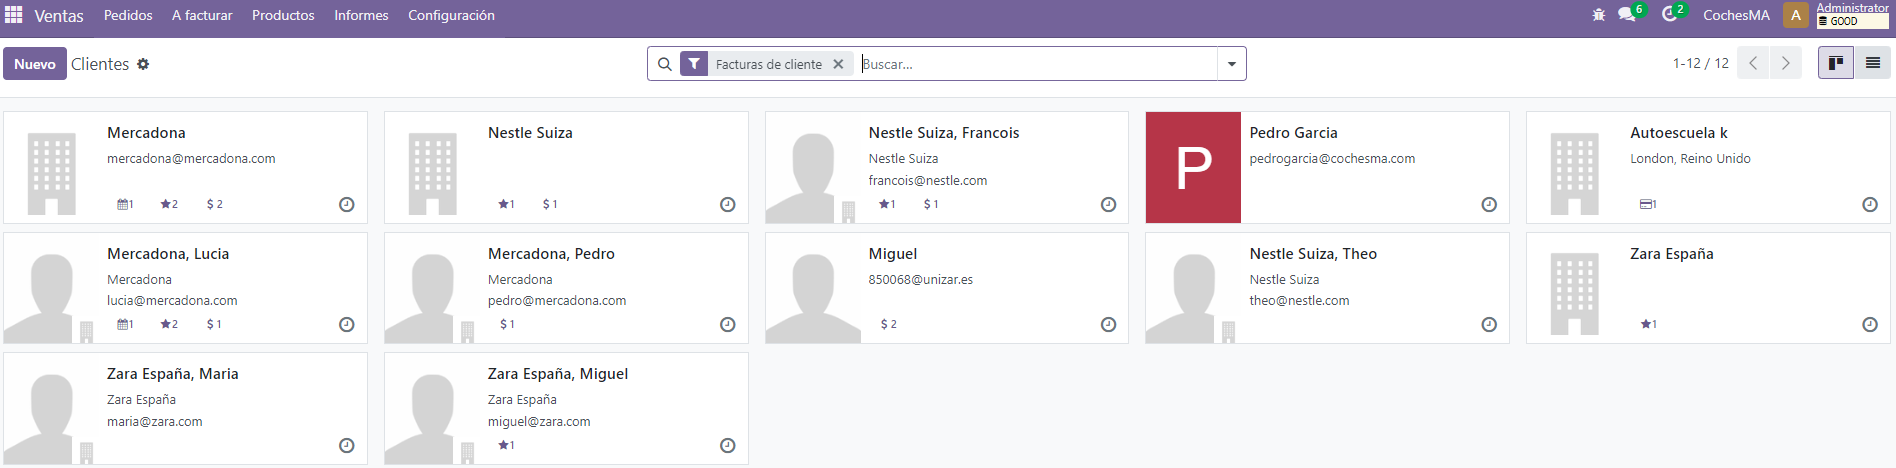
\includegraphics[width=1\linewidth]{fotosRelacion/clientes.png}
    \caption{Lista de clientes de la compañía con sus respectivos contactos}
    \label{fig:enter-label}
\end{figure}
\paragraph{}    
En este proceso se han creado 2 iniciativas para dos clientes interesados. Se ha creado un presupuesto para uno de ellos. Finalmente, en una segunda revisión del presupuesto se ha aplicado un descuento del 5\% de descuento sobre el precio y se ha cerrado el acuerdo de venta.
\begin{figure}[h]
    \centering
    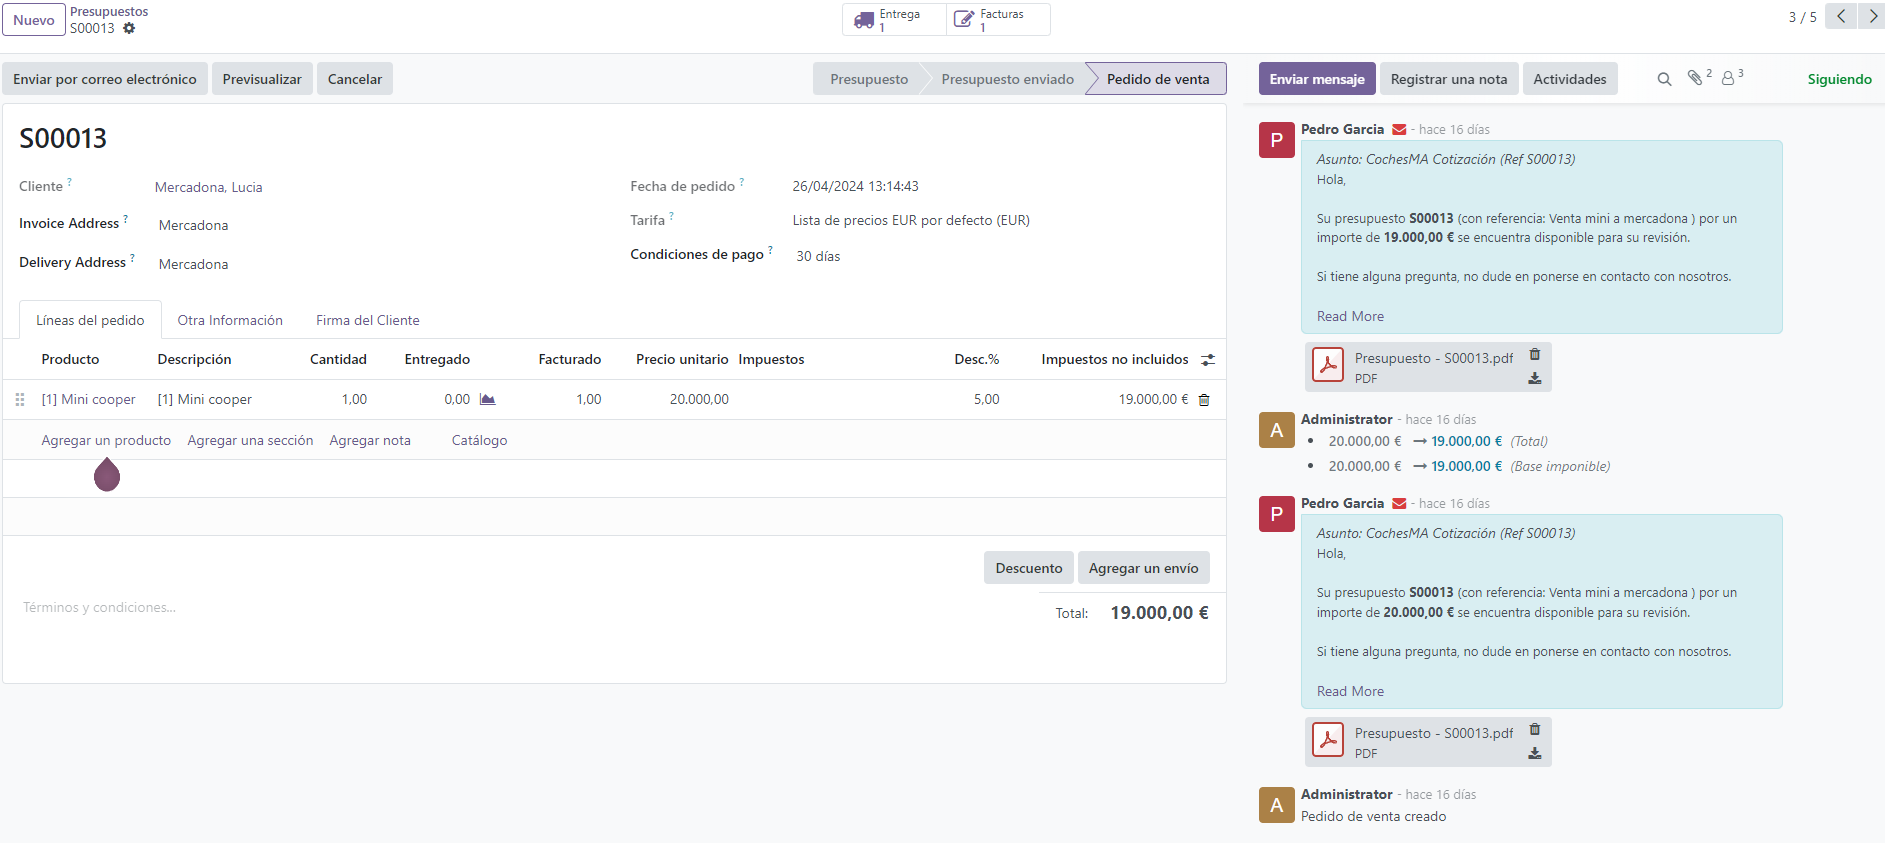
\includegraphics[width=1\linewidth]{fotosRelacion/presupuesto.png}
    \caption{Presupuesto de la venta}
    \label{fig:enter-label}
\end{figure}
Este proceso también está sincronizado con el módulo de Facturación por lo que el estado de la venta se puede observar desde la siguiente vista.
\newpage
\begin{figure}[h]
    \centering
    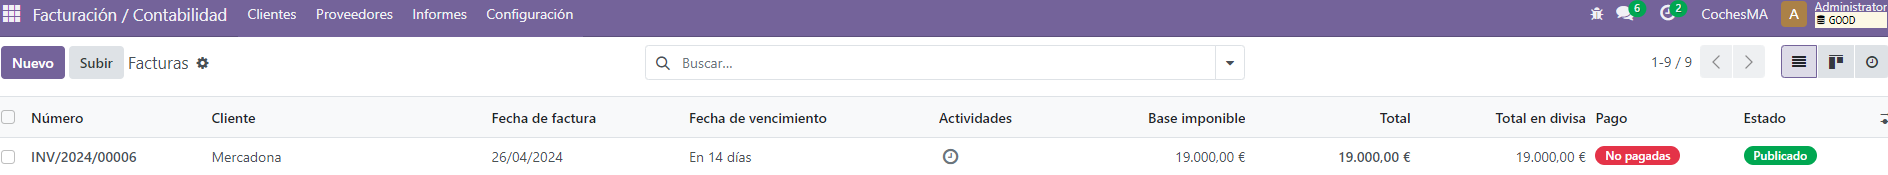
\includegraphics[width=1\linewidth]{fotosRelacion/facturacion.png}
    \caption{Lista de las ventas desde el módulo de Facturación}
    \label{fig:enter-label}
\end{figure}
Durante todo el proceso de venta se ha ido actualizando la vista Kanban del módulo \textit{CRM} que permite una vista general del estado de las iniciativas y ventas.
\begin{figure}[h]
    \centering
    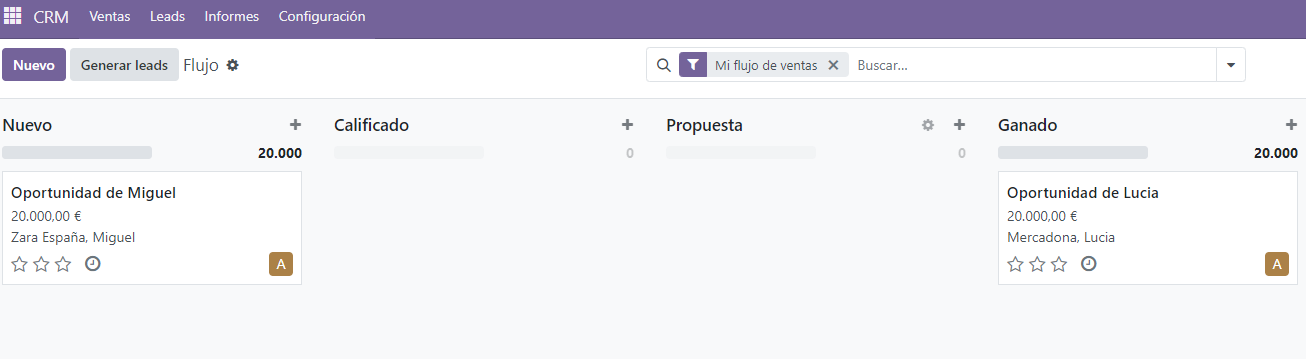
\includegraphics[width=1\linewidth]{fotosRelacion/kanban.png}
    \caption{Vista Kanban del flujo de ventas del módulo CRM}
    \label{fig:enter-label}
\end{figure}
Por último, se ha realiza un BPMN sobre el proceso de venta.
\begin{figure}[h]
    \centering
    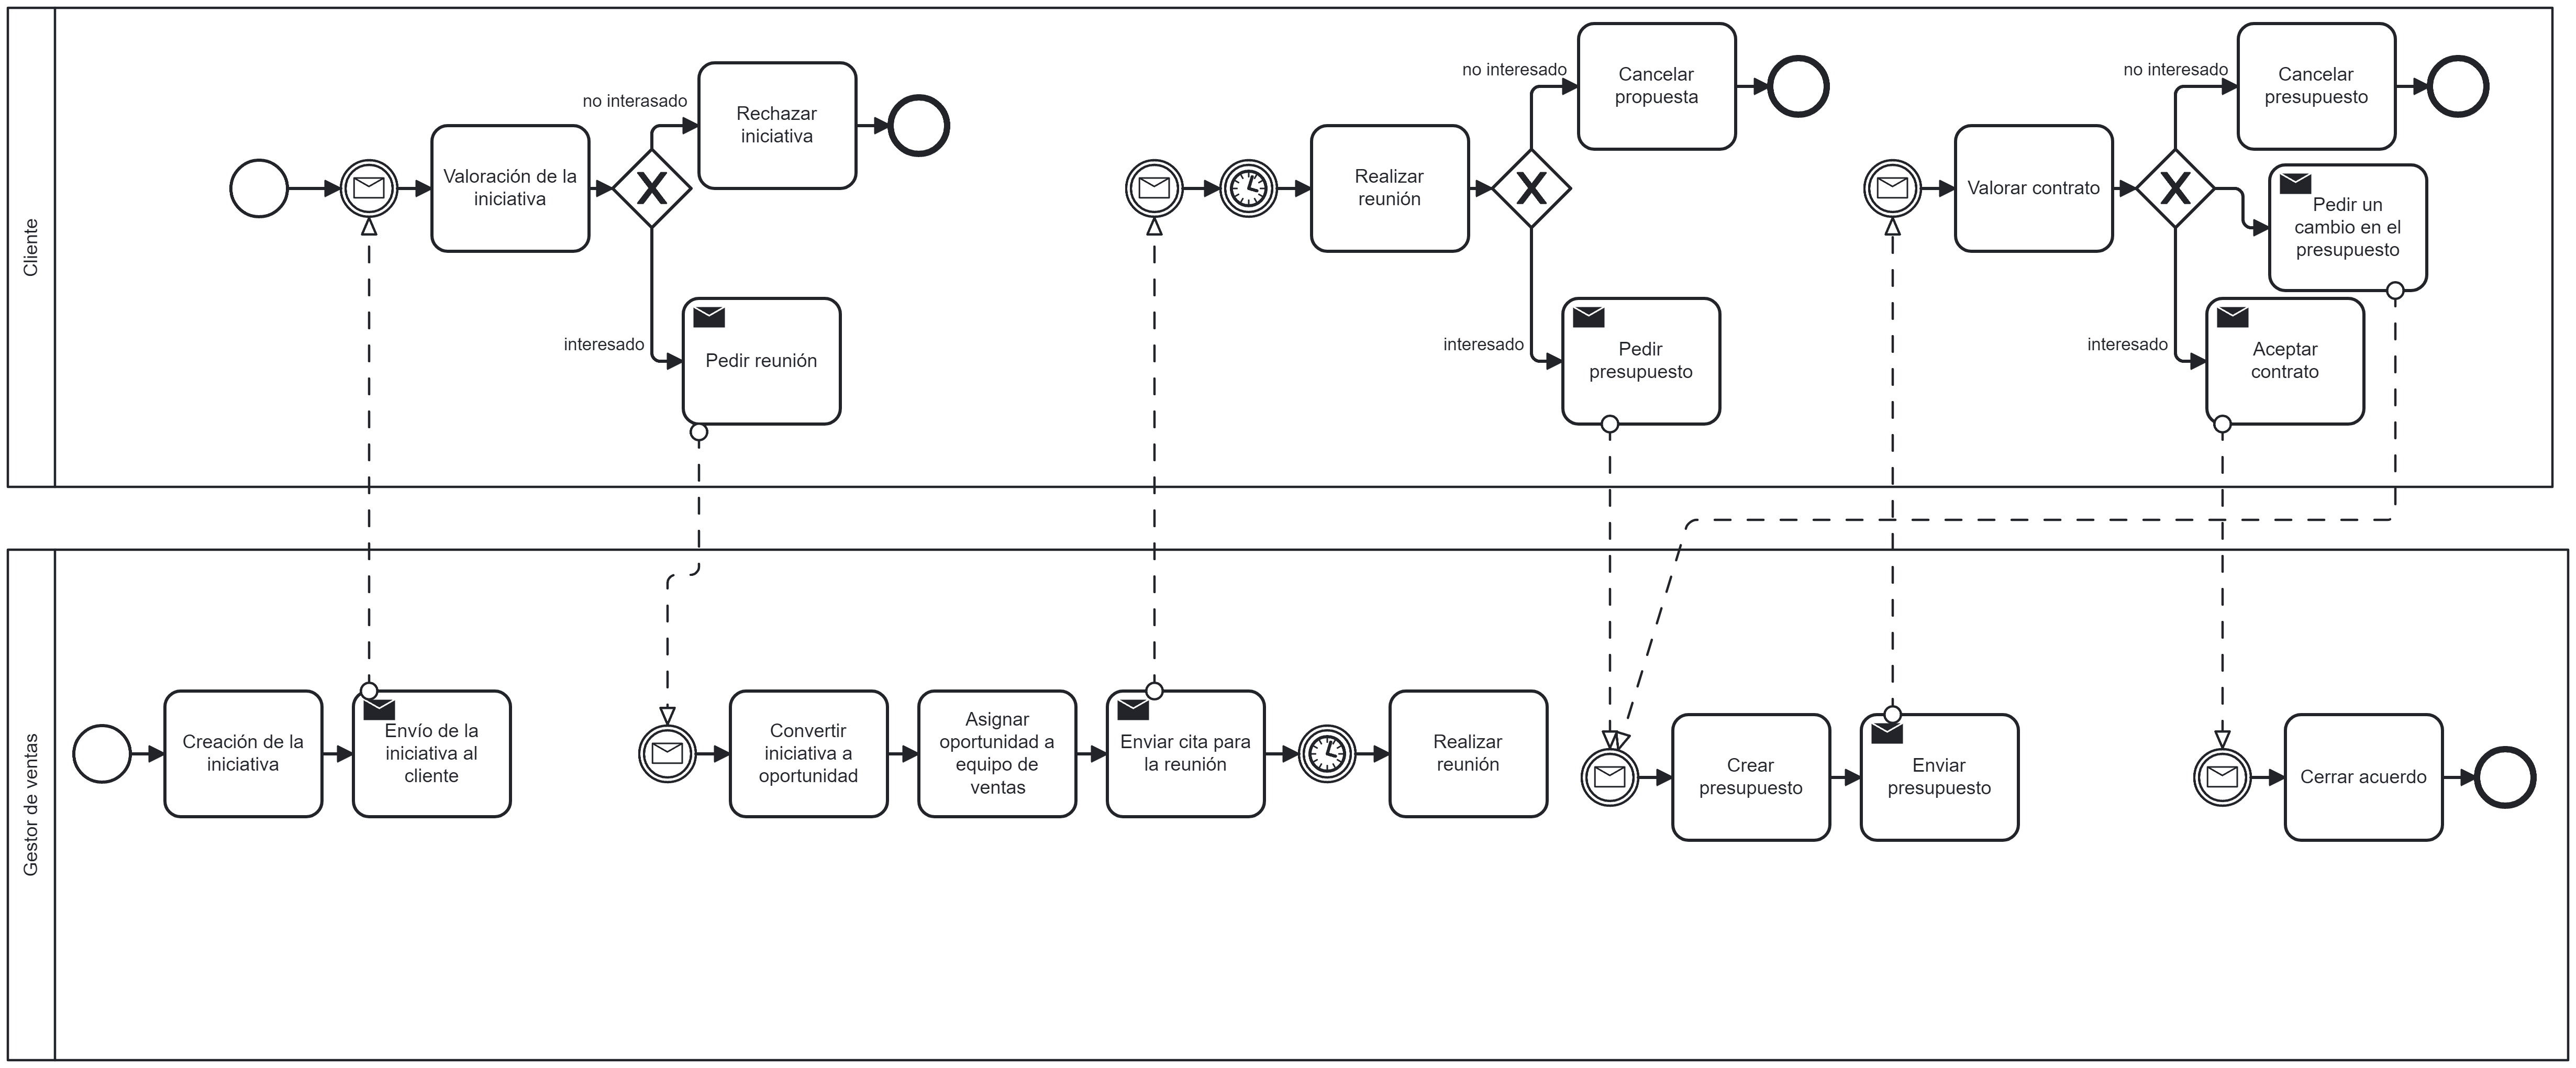
\includegraphics[width=1\linewidth]{bpmn/venta.png}
    \caption{BPMN del proceso de venta}
    \label{fig:enter-label}
\end{figure}
\subsection{Conclusiones}
\paragraph{}
La solución que ofrece Odoo para estas funcionalidades las cubre mediante el módulo \textit{CRM}, \textit{Ventas} y \textit{Facturación}. De esta manera se permite gestionar de manera eficiente la relación con los clientes y gestionar el proceso de ventas y facturación. La configuración de estos módulos es relativamente simple, y una vez realizado, proporciona una plataforma sólida para cubrir la gestión de clientes, oportunidades de negocio, presupuestos y facturas.
\paragraph{}
Se ha demostrado como se ha utilizado de forma efectiva las herramientas disponibles para llevar a cabo la generación de leads, la creación de presupuestos y facturas mediante Odoo. Además, gracias a la integración del correo electrónico en la sección de Configuración técnica se facilita la comunicación con los clientes y la transferencia de presupuestos y facturas.
\paragraph{}
En este apartado se ha evaluado la capacidad de Odoo para la gestión de relaciones con los clientes y las ventas. Se ha confirmado que Odoo ofrece una plataforma completa para llevar a cabo esta gestión, permite una configuración flexible y capacidad para optimizar la gestión comercial de la compañía. En resumen, tiene una correcta implementación de módulos para llevar a cabo la relación con los clientes y desarrollar los procesos de venta mediante Odoo. 